\documentclass[CJKmath,a4paper,10pt]{ctexart}
\usepackage{geometry}
\geometry{inner=1.5cm,outer=1.5cm,top=2.45cm,bottom=1cm}
\usepackage[dvipsnames,svgnames,x11names,table]{xcolor}


\RequirePackage{amssymb} % Must be loaded before unicode-math
\RequirePackage{unicode-math} % Math fonts in xetexorluatex
%\setmathfont{texgyrepagella-math.otf}
%\setmainfont{STIXTwoText}[
%	Path=./fonts/STIXTwoText/,
%  Extension = .otf,
%  UprightFont = STIXTwoMath-Regular,
%  BoldFont = STIXTwoText-SemiBold,
%  ItalicFont = STIXTwoText-Italic,
%  BoldItalicFont = STIXTwoText-BoldItalic,
%]
%\setmathfont{STIXTwoMath-Regular.otf}

\usepackage{tikz,calc}
\usetikzlibrary{calc,arrows,shadows.blur,tikzmark}
% By default all math in TikZ nodes are set in inline mode. Change this to
% displaystyle so that we don't get small fractions.
\everymath{\displaystyle}

\usepackage[most]{tcolorbox}
\tcbuselibrary{breakable, skins,theorems}


\usepackage{xkeyval}
\makeatletter 
\usepackage{amsmath,amssymb,amsthm}
\usepackage{xkeyval} 
\usepackage{zhlipsum}
\tcbset{
    common/.style={
      fontupper=\rmfamily,
      lower separated=true,
      coltitle=black,
      colback=gray!5,
      boxrule=0.5pt,
      fonttitle=\bfseries,
      enhanced,
      breakable,
      top=8pt,
      before skip=8pt,
      attach boxed title to top left={yshift=-0.05in,xshift=0.15in},
      boxed title style={
      	boxrule=0pt,
        colframe=black,
        arc=0pt,
        outer arc=0pt,
        drop fuzzy shadow
     	},
      separator sign={.},
      drop fuzzy shadow
     },
     litistyle/.style={  %例题风格
     	common,
      colframe=gray,% 
      colback=white,
      colbacktitle=Gold,
      sharp corners,rounded corners=southeast,
      overlay unbroken and last={
      \node[anchor=south east, outer sep=0pt] at (\linewidth-width,0){\textcolor{black!60}{$\blacksquare$}};}
         },
% -----------------------------------------------------------------------------
% Explanation: BreakableBox@title key
% The following defines a pgfkeys/tcolorbox key named
%   "BreakableBox@title" which accepts 2 arguments (see 
%   "/.code n args={2}"). When the key is used like
%   "BreakableBox@title={<env>}{<optTitle>}" the code below is executed
%   with #1=<env> and #2=<optTitle>.
%
% Purpose:
% - If the second argument (#2) is empty, set the tcolorbox title to
%     \csname <env>name\endcsname~\thetcbcounter
%   which expands to the environment name (e.g. "liti" -> \litiname)
%   followed by the current counter value.
% - If the second argument is provided, append " (#2)" to the title.
%
% Notes:
% - This relies on \makeatletter being active so that keys with '@'
%   are allowed in control sequence names.
% - \ifblank is used to test whether #2 is empty; ensure the package
%   that provides \ifblank (for example, etoolbox or xparse) is loaded
%   earlier if necessary.
% - Example usage inside the code: \tcbset{title={...}} sets the
%   tcolorbox title key accordingly.
%
         BreakableBox@title/.code n args={2}
              {
                \ifblank{#2}
                  {\tcbset{title={\csname #1name\endcsname~\thetcbcounter}}}
                  {\tcbset{title={\csname #1name\endcsname~\thetcbcounter\ (#2)}}}
              },
}      
  % define an internal control sequence \newbreakablebox for fancy mode's newtheorem
  % #1 is the environment name, #2 is the prefix of label, #3 is the style
  % style: thmstyle, defstyle, prostyle
  % e.g. \newbreakablebox{theorem}{thm}{thmstyle}
  % will define two environments: numbered ``theorem'' and no-numbered ``theorem*''
  % WARNING FOR MULTILINGUAL: this cs will automatically find \theoremname's definition,
  % WARNING FOR MULTILINGUAL: it should be defined in language settings.
  \newcommand{\newbreakablebox}[3]{
    \ifcsundef{#1name}{%
      % define a default name if not defined before
      \tcbset{BreakableBox@title/.code n args={2}{\tcbset{title={use newcommand define #1name}}} }
    }{\relax}
    \DeclareTColorBox[auto counter,number within=section]{#1}{ g o t\label g }{
        common, % use common style
        #3, % use the style passed in
        IfValueTF={##1}
          {BreakableBox@title={#1}{##1}}
          {
            IfValueTF={##2}
            {BreakableBox@title={#1}{##2}}
            {BreakableBox@title={#1}{}}
          },
        IfValueT={##4}
          {
            IfBooleanTF={##3}
              {label={##4}}
              {VIVID@label={#2}{##4}}
          }
      }
    \DeclareTColorBox{#1*}{ g o }{
        common,#3,
        IfValueTF={##1}
          {BreakableBox@title={#1}{##1}}
          {
            IfValueTF={##2}
            {BreakableBox@title={#1}{##2}}
            {BreakableBox@title={#1}{}}
          },
      }
  }
  % define several environment 
  % we define headers like \definitionname before
  \newcommand{\litiname}{例题}
  \newbreakablebox{liti}{def}{litistyle}
  
  
%补充内容
%%设置新字体
%%定义带圈数字命令
\newfontfamily{\nmfont}{circlenumber}
[%
Extension=.otf,
Path=./fonts/]

\newcommand{\quan}[1]{{\nmfont \symbol{#1}}}
\newcommand{\kk}[1]{\quan{\numexpr32+#1}}%\kk{<参数范围1-95>}96、97、98、99分别用\quan{196} \quan{197} \quan{199} \quan{201}

%脚注使用带圈数字
\newcommand*\kkctr[1]{%
  \protect\kk{\number\numexpr\value{#1}\relax}}
\renewcommand*\thefootnote{\textcolor{black}{\kkctr{footnote}}}

%%无悬挂脚注格式
\renewcommand\@makefntext[1]{%
  \setlength\parindent{2\ccwd}\selectfont
  \@thefnmark\ #1}

%修改\part，使其不分页
\def\@endpart{%
	\thispagestyle{empty}
  \vskip40\p@%
   \@afterheading}



\RequirePackage{enumitem}
%\newenvironment{myenum}{\begin{enumerate}[label=\protect\kk{\arabic*}]\small}{\end{enumerate}}%
\setlist{noitemsep}
\setlist[enumerate, 1]{label=\protect\kk{\arabic*},itemsep=0.5ex}  
\makeatother



%%%marker环境
\newtcolorbox{marker}[1][]{enhanced,before skip=2mm,
	after skip=3mm,fontupper=\rmfamily,
	boxrule=0.4pt,left=5mm,right=2mm,top=1mm,bottom=1mm,
	colback=yellow!50,colframe=yellow!20!black,
	sharp corners,rounded corners=southeast,
	arc is angular,arc=3mm,underlay={%
		\path[fill=tcbcolback!80!black] ([yshift=3mm]interior.south east)--++(-0.4,-0.1)--++(0.1,-0.2);
		\path[draw=tcbcolframe,shorten <=-0.05mm,shorten >=-0.05mm] ([yshift=3mm]interior.south east)--++(-0.4,-0.1)--++(0.1,-0.2);
		\path[fill=yellow!50!black,draw=none] (interior.south west) rectangle node[white]{\Huge\bfseries !} ([xshift=4mm]interior.north west);
	},
	drop fuzzy shadow,#1
}


\usepackage{graphicx}
\usepackage{float}
\begin{document}



\section{解答题}
\begin{liti}
已知函数 \( f_k(x) = \cos^{2k}x - \sin^{2k}x \)，\( g_k(x) = \cos^{2k}x + \sin^{2k}x \)（\( k \in \mathbb{N}^* \)），则下列说法正确的是（\quad）
\begin{enumerate}[label=\textbf{\Alph*}]
	\item 函数 \( f_1(x) \) 在 \( \left[0, \frac{\pi}{2}\right] \) 上单调递减
	\item 函数 \( g_2(x) \) 的最小正周期为 \( \frac{\pi}{2} \)
	\item 函数 \( g_3(x) \) 的值域为 \( \left[\frac{1}{4}, 1\right] \)
	\item 函数 \( f_4(x) \) 的图象关于 \( x = \frac{\pi}{4} \) 对称
\end{enumerate}
\tcblower
\textbf{解：}
\begin{itemize}
	\item \textbf{A}：当 $ k=1 $ 时，$ f_1(x) = \cos^2 x - \sin^2 x = \cos 2x $。当 $ x \in \left[0, \frac{\pi}{2}\right] $ 时，$ 2x \in [0, \pi] $，函数 $ y = \cos t $ 在 $ [0, \pi] $ 上单调递减，所以 $ f_1(x) $ 在 $ \left[0, \frac{\pi}{2}\right] $ 上单调递减，故 A 正确；
	
	\item \textbf{B}：当 $ k=2 $ 时，$ g_2(x) = \cos^4 x + \sin^4 x = (\cos^2 x + \sin^2 x)^2 - 2\sin^2 x \cos^2 x = 1 - \frac{1}{2}\sin^2 2x = 1 - \frac{1}{2} \cdot \frac{1-\cos 4x}{2} = \frac{3}{4} + \frac{1}{4}\cos 4x $，其最小正周期 $ T = \frac{2\pi}{4} = \frac{\pi}{2} $，故 B 正确；

	\item \textbf{C}：当 $ k=3 $ 时，$ g_3(x) = \cos^6 x + \sin^6 x = (\cos^2 x + \sin^2 x)(\cos^4 x - \cos^2 x \sin^2 x + \sin^4 x) = 1 \cdot \big[(\cos^2 x + \sin^2 x)^2 - 3\sin^2 x \cos^2 x \big] = 1 - \frac{3}{4}\sin^2 2x $。
因为 $ 0 \le \sin^2 2x \le 1 $，所以 $ g_3(x) \in \left[1 - \frac{3}{4}, 1\right] = \left[\frac{1}{4}, 1\right] $，故 C 正确；

	\item \textbf{D}：当 $ k=4 $ 时，$ f_4(x) = \cos^8 x - \sin^8 x $。
若函数图象关于 $ x = \frac{\pi}{4} $ 对称，则应有 $ f_4\left(\frac{\pi}{4}-x\right) = f_4\left(\frac{\pi}{4}+x\right) $。
取特值检验：令 $ x = \frac{\pi}{4} $，则需检验 $ f_4(0) $ 与 $ f_4\left(\frac{\pi}{2}\right) $ 是否相等。
因为 $ f_4(0) = \cos^8 0 - \sin^8 0 = 1 $，$ f_4\left(\frac{\pi}{2}\right) = \cos^8 \frac{\pi}{2} - \sin^8 \frac{\pi}{2} = -1 $，
显然 $ f_4(0) \ne f_4\left(\frac{\pi}{2}\right) $，所以 $ f_4(x) $ 的图象不关于 $ x = \frac{\pi}{4} $ 对称，故 D 错误。
\end{itemize}
故选：\textbf{ABC}。

\end{liti}
\begin{liti}
	如图1所示，平板小车$A$置于光滑水平平台上，在小车左端放有一可视为质点的物块$B$，将重物$C$用不可伸长的轻绳跨过光滑的滑轮与小车连接，系统保持静止。重物$C$距地面的高度$H=5.75\mathrm{m}$，物块与重物的质量均为$m=1\mathrm{kg}$，小车到定滑轮距离足够远。现由静止释放小车，同时给物块以$v_0=4\mathrm{m/s}$的水平向右的初速度，此后至重物落地前小车的速度-时间图像如图2所示，此间物块$B$未脱离小车，重力加速度$g$取$10\mathrm{m/s^2}$。试求：
	\begin{enumerate}[label=(\arabic*)]
		\item 物块与小车间的动摩擦因数$\mu$及小车的质量$M$；
		\item 重物落地时，物块相对小车的位置；
		\item 小车长度的最小值$L_0$。
	\end{enumerate}
	
	% TikZ绘制图1和图2

\end{liti}	
	\begin{figure}[htbp]
	\centering
	\begin{minipage}{0.55\textwidth}
		\centering
		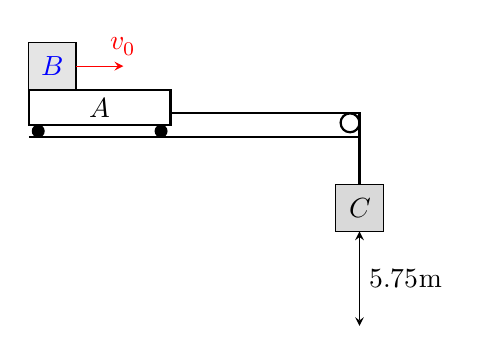
\begin{tikzpicture}[>=stealth, scale=0.6]
			% 水平平台
			\draw[thick] (0,0) -- (7,0);
			% 小车A
			\draw[thick] (0,0.25) rectangle (3,1) node[midway] {$A$};
			\draw[fill=black](0.2,0.125) circle(0.125);
			\draw[fill=black](2.8,0.125) circle(0.125);
			% 物块B
			\draw[fill=gray!20] (0,1) rectangle (1,2) node[midway,blue] {$B$};
			% 定滑轮
			\draw[thick] (6.8,0.3) circle (0.2) node[right] {\ \ 定滑轮};
			% 轻绳
			\draw[thick] (3,0.5) -- (7,0.5) -- (7,-1);
			% 重物C
			\draw[fill=gray!30] (6.5,-1) rectangle (7.5,-2) node[midway] {$C$};
			% 高度H
			%\draw[dashed] (7,0) -- (7,4) node[midway,right] {$H$};
			%\draw (7,0) -- (7.8,0) node[right] {$0$};
			\draw[<->] (7,-2) -- (7,-4) node[right,midway] {$5.75\mathrm{m}$};
			% 初速度v0
			\draw[->,red] (1,1.5) -- (2,1.5) node[above] {$v_0$};
			% 标注光滑平台
			\node at (4,-0.5) {光滑水平平台};
		\end{tikzpicture}
		\caption{图1}
	\end{minipage}
	\begin{minipage}{0.4\textwidth}
		\centering
		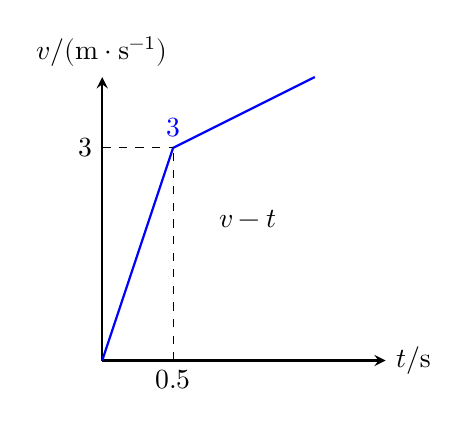
\begin{tikzpicture}[>=stealth, scale=0.9]
			% 坐标轴
			\draw[thick,->] (0,0) -- (4,0) node[right] {$t/\mathrm{s}$};
			\draw[thick,->] (0,0) -- (0,4) node[above] {$v/(\mathrm{m\cdot s^{-1}})$};
			% 刻度
			\draw (1,0) node[below] {$0.5$};
			\draw (0,3) node[left] {$3$};
			% v-t图像：0到0.5s是直线，之后斜率变小的直线
			\draw[thick,blue] (0,0) -- (1,3) node[above] {$3$}--(3,4);
			\draw[dashed] (1,0) -- (1,3);
			\draw[dashed] (0,3) -- (1,3);
			% 标注
			\node at (2,2) {小车的$v-t$图像};
		\end{tikzpicture}
		\caption{图2}
	\end{minipage}
\end{figure}

\textbf{解：}
\begin{enumerate}[label=(\arabic*)]
	\item 由图2可知，在 $ 0 \sim 0.5\,\mathrm{s} $ 内，小车加速运动，加速度 $ a_{A1} = \dfrac{3-0}{0.5} = 6\,\mathrm{m/s^2} $。
	设 $ t=0.5\,\mathrm{s} $ 时物块与小车共速，此时 $ v_A = v_B = 3\,\mathrm{m/s} $。
	物块做匀减速运动，$ v_B = v_0 - \mu g t $，代入数据得 $ 3 = 4 - \mu \cdot 10 \cdot 0.5 $，解得 $ \mu = 0.2 $。
	此时对\textbf{小车和重物}整体分析（物块相对小车向右滑，对小车摩擦力向右）：
	$ m_C g + \mu m_B g = (M + m_C) a_{A1} $，
	即 $ 10 + 2 = (M+1) \cdot 6 $，解得 $ M = 1\,\mathrm{kg} $。
	\begin{marker}\footnotesize
		连接体的核心是加速度相等，即此时重物和小车加速度相等。此时水平方向受的合外力为重力+物块B给予的摩擦力，即上式左边。
	\end{marker}
	如果不理解也可以逐个受力分析：设绳子的拉力为$T$，则：\\
	\begin{minipage}{0.5\textwidth}
				\begin{figure}[H]
					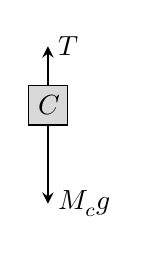
\begin{tikzpicture}[>=stealth,scale=0.5]
						% 重物C
						\draw[fill=gray!30] (0,0) rectangle (1,1) node[midway] {$C$};
						\draw[thick,->] (0.5,0) -- (0.5,-2) node[right] {$M_cg$};
						\draw[thick,->] (0.5,1) -- (0.5,2) node[right] {$T$};
					\end{tikzpicture}
				\end{figure}
	\end{minipage}	
	\begin{minipage}{0.5\textwidth}
		\begin{figure}[H]
			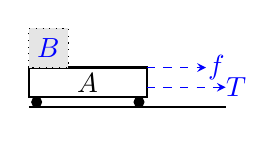
\begin{tikzpicture}[>=stealth,scale=0.5]
				\draw[thick] (0,0.25) rectangle (3,1) node[midway] {$A$};
				\draw[fill=black](0.2,0.125) circle(0.125);
				\draw[fill=black](2.8,0.125) circle(0.125);
				% 物块B
				\draw[fill=gray!20,dotted] (0,1) rectangle (1,2) node[midway,blue] {$B$};
				%拉力
				\draw[dashed,blue,->,thin] (3,0.5) -- (5,0.5)node{$\ \ T$};
				%摩擦力
				\draw[dashed,blue,->,thin] (3,1) -- (4.5,1)node{$\ \ f$};
				\draw[thick] (0,0) -- (5,0);
				\node at (2,-0.5) {\footnotesize\bfseries 光滑水平平台};
			\end{tikzpicture}
		\end{figure}
	\end{minipage}
	$T$是绳子的内部拉力，$f$是物块B给予的摩擦力。则有
	\begin{align*}
		&M_cg-T=M_ca_{A1}=M_c\times 6\iff T= 4\\
		&T+f=M_A\times a_{A1}\\
		&代入T=4，f=2,a_{A1}=6得：M_A=1
	\end{align*}
	\item 共速后，假设物块与小车相对滑动。
	对小车和重物整体（物块相对小车向左滑，对小车摩擦力向左）：
	$ m_C g - \mu m_B g = (M + m_C) a_{A2} $，
	即 $ 10 - 2 = (1+1) a_{A2} $，解得 $ a_{A2} = 4\,\mathrm{m/s^2} $。
	对物块：$ \mu m_B g = m_B a_{B2} $，得 $ a_{B2} = 2\,\mathrm{m/s^2} $。
	因 $ a_{A2} > a_{B2} $，假设成立，小车速度将超过物块。
	第一阶段（$0 \sim 0.5\,\mathrm{s}$）小车位移 $ x_{A1} = \frac{1}{2} a_{A1} t_1^2 = 0.75\,\mathrm{m} $。
	剩余下落高度 $ h = 5.75 - 0.75 = 5\,\mathrm{m} $。
	设第二阶段时间为 $ t_2 $，则 $ h = v_1 t_2 + \frac{1}{2} a_{A2} t_2^2 $，即 $ 5 = 3 t_2 + 2 t_2^2 $，解得 $ t_2 = 1\,\mathrm{s} $。
	此阶段物块位移 $ x_{B2} = v_1 t_2 + \frac{1}{2} a_{B2} t_2^2 = 3 + 1 = 4\,\mathrm{m} $，小车位移 $ x_{A2} = 5\,\mathrm{m} $。
	第二阶段物块相对小车位移 $ \Delta x_2 = x_{B2} - x_{A2} = -1\,\mathrm{m} $（向左）。
	第一阶段物块位移 $ x_{B1} = v_0 t_1 - \frac{1}{2} \mu g t_1^2 = 4 \times 0.5 - 0.25 = 1.75\,\mathrm{m} $。
	第一阶段相对位移 $ \Delta x_1 = x_{B1} - x_{A1} = 1\,\mathrm{m} $（向右）。
	总相对位移 $ \Delta x = \Delta x_1 + \Delta x_2 = 0\,\mathrm{m} $。
	即重物落地时，物块相对小车位置回到左端。
	
	\item 过程最大相对位移为 $ t=0.5\,\mathrm{s} $ 时的 $ \Delta x_1 = 1\,\mathrm{m} $，此后物块相对后退。
	为使物块不脱离小车，小车长度至少为 $ 1\,\mathrm{m} $。
\end{enumerate}

\textbf{解答概要：}
\begin{enumerate}
    \item \textbf{第一阶段 ($0\sim 0.5\,\mathrm{s}$)}：利用 $v-t$ 图像求出小车加速度 $a_{A1}=6\,\mathrm{m/s^2}$，结合共速条件求出动摩擦因数 $\mu=0.2$，再由系统牛顿第二定律求出小车质量 $M=1\,\mathrm{kg}$。
    \item \textbf{第二阶段 ($t>0.5\,\mathrm{s}$)}：共速后摩擦力反向，分别求出小车和物块的新加速度，计算剩余下落高度 $5\,\mathrm{m}$ 所需时间 $1\,\mathrm{s}$。通过位移差计算得出重物落地时物块刚好回到小车左端。
    \item \textbf{小车长度}：根据最大相对位移 $\Delta x_{\max}=1\,\mathrm{m}$ 确定小车最小长度 $L_0=1\,\mathrm{m}$。
\end{enumerate}

\end{document}